% =====================================================================
% Revised Section 3 (Methods) and Section 4 (Experiments / Results)
% Drop-in replacement for the draft's Sections 3-4.
% Requires: \usepackage{booktabs, graphicx, xcolor, amsmath}
% Citation keys below are placeholders; match them to your .bib:
%   peebles2023dit, choudhury2025apt, kim2026ddit, hu2022lora, anagnostidis2025flexidit
% Red TODOs mark results from the queued follow-ups (A, B, Stage 0).
% =====================================================================
\newcommand{\todo}[1]{\textcolor{red}{[\textbf{TODO:} #1]}}

\section{Methods}
\label{sec:methods}

All adapted conditions use \emph{one} shared model and differ only in the patch-size schedule applied at sampling time.

\subsection{Mixed-scale tokenization}
\label{sec:tokenization}
We start from a pretrained class-conditional DiT-S/2~\citep{peebles2023dit} (32.96M parameters) on the $32{\times}32{\times}4$
VAE latent of ImageNet-256. The latent is partitioned into $B{=}16$ non-overlapping blocks of $8{\times}8$ latent cells.
At denoising step $t$, block $b$ is tokenized with patch size $p_{b,t}\in\{2,4,8\}$, contributing $16$, $4$, or $1$ tokens, so
\begin{equation}
N_t=\sum_{b=1}^{16}\left(\frac{8}{p_{b,t}}\right)^2 \in [16, 256].
\label{eq:tokens}
\end{equation}
All tokens of an image form one sequence; images with different $N_t$ in a batch are padded and masked in attention.
Each patch size has its own input embedding and output de-embedding. Patch size 2 reuses the frozen pretrained layers.
The $p{=}4$ and $p{=}8$ embeddings are initialized as the pretrained embedding applied to the average-pooled patch, and their
de-embeddings as a nearest-neighbour upsampling of the pretrained $2{\times}2$ head. Coarse tokens receive a learned patch-size
embedding. Because DiT uses fixed 2D sin-cos positions, we evaluate them exactly at each coarse patch's centre rather than interpolating.

\subsection{Adapting the pretrained model}
\label{sec:adaptation}
We add rank-32 LoRA~\citep{hu2022lora} to the attention (\texttt{qkv}, \texttt{proj}) and MLP (\texttt{fc1}, \texttt{fc2}) linears of all
12 blocks, and apply the low-rank update \emph{only to coarse tokens}. Fine tokens therefore pass through unmodified weights, and an
all-fine layout reproduces the frozen teacher exactly (verified to numerical precision).

Two further components, applied only in coarse regions, proved necessary (Table~\ref{tab:ablation}):
\begin{itemize}
  \item \textbf{Noise skip.} At high noise the target is close to the input ($\epsilon\approx x_t$), and a coarse token cannot pass
  per-pixel noise back through the pretrained trunk. Coarse regions therefore predict
  \begin{equation}
  \hat\epsilon=\sqrt{1-\bar\alpha_t}\,x_t+\sqrt{\bar\alpha_t}\,h,
  \label{eq:skip}
  \end{equation}
  where $h$ is the coarse head's output.
  \item \textbf{Fine-grid decoder.} A small convolutional decoder (1$\times$1, 3$\times$3, 1$\times$1 convolutions, conditioned on
  $(t,y)$, zero-initialized) reads, for every $2{\times}2$ cell, the coarse trunk feature covering it and the frozen \emph{fine}
  patch embedding of $x_t$. It adds a per-cell correction to $h$, restoring detail the coarse token cannot carry.
\end{itemize}
The base DiT and VAE stay frozen; 3.29M parameters are trained. As a pre-specified fallback, we also trained a full fine-tune of the
trunk (Section~\ref{sec:training-results}).

\subsection{Self-distillation}
\label{sec:distillation}
The adapted model $\epsilon_{\theta_L}$ is trained to match the frozen teacher $\epsilon_{\theta_T}$ on the same latent:
\begin{equation}
\mathcal{L}=\big\|\epsilon_{\theta_L}(x_t,t,y;\,\mathbf{p})-\epsilon_{\theta_T}(x_t,t,y)\big\|_2^2
+0.1\,\big\|\Sigma_{\theta_L}-\Sigma_{\theta_T}\big\|_2^2,
\label{eq:loss}
\end{equation}
where $\mathbf{p}$ is the patch layout and $\Sigma$ the learned-variance channels. No external images are used. The teacher generates
50,000 CFG-4 samples with classes drawn uniformly from all 1,000 classes, and stores 5,000 complete 50-step DDIM trajectories.

Each batch of 256 is half real trajectory states and half final samples re-noised at uniform $t\in[0,999]$. 10\% of labels are
replaced by the null class, so the unconditional CFG branch is also distilled.

Layouts are drawn per image as follows:
\begin{itemize}
  \item uniform $p{=}4$ (15\%) or uniform $p{=}8$ (15\%);
  \item spatially smooth random fields over $\{2,4,8\}$;
  \item for trajectory states, the exact masks the inference scheduler produces (Eq.~\ref{eq:schedule}) at random thresholds, so the
  model trains on the layouts it will see at inference.
\end{itemize}
We train for 60 minutes (12,585 steps) with AdamW (learning rate $3{\times}10^{-4}$, cosine decay) in bf16.

\subsection{Selection signal and schedules}
\label{sec:schedules}
Following DDiT~\citep{kim2026ddit}, the signal is the third-order finite difference of the latent trajectory,
$\Delta^3 z_t=z_t-3z_{t-1}+3z_{t-2}-z_{t-3}$, but computed per block. For a candidate size $p$, we take the spatial standard deviation
of $\Delta^3 z_t$ in each $p{\times}p$ window, average it over channels, and take the 75th percentile over the block's windows to get
$s^{(p)}_{b,t}$. The scheduler picks the coarsest size whose score is below a threshold:
\begin{equation}
p_{b,t}=\max\{p\in\{2,4,8\}: s^{(p)}_{b,t}<\tau\}\quad(\text{default }2).
\label{eq:schedule}
\end{equation}
$\Delta^3$ needs four latents, so the first three steps always run at $p{=}2$.
Table~\ref{tab:arms} defines the compared conditions. We calibrate $\tau$ separately for the temporal and joint schedules to hit target
budgets of about 200, 150, and 100 mean tokens per step.

\begin{table}[t]
\centering
\small
\caption{Compared conditions. All adapted conditions run the same checkpoint.}
\label{tab:arms}
\begin{tabular}{p{3.0cm}p{9.6cm}}
\toprule
Condition & Definition \\
\midrule
Teacher, $S$ steps & Frozen DiT-S/2, DDIM with $S\in\{50,40,33,25,20,15,10\}$ (fewer-steps baseline). \\
Uniform $p$ & All blocks at $p\in\{4,8\}$ after warm-up. \\
Fixed switch & $p{=}4$ for the first $k$ scheduled steps, then $p{=}2$. \\
Temporal (DDiT-style) & One $p$ per step for the whole image: Eq.~\ref{eq:schedule} on the image-mean score. \\
Spatial (fixed) & Blocks ranked by their first-scheduled-step score and coarsened in rank order ($p{=}4$, then $p{=}8$) up to the
token budget; the mask is then held fixed (causal). \\
Joint (ours) & Eq.~\ref{eq:schedule} per block, per step. \\
Spatial / joint random & The same per-image (and per-step) multiset of patch sizes placed on random blocks. Matches the token count
and isolates the value of the selection signal. \\
\bottomrule
\end{tabular}
\end{table}

\subsection{Allocation gap}
\label{sec:gap}
To evaluate a signal independently of the schedule, we force a single block to $p$ for all scheduled steps (all others fine) and record
the LPIPS increase against the teacher's image. Repeating this for all 16 blocks gives a per-image damage map. The allocation gap is
$(1-\rho_S)/2$, where $\rho_S$ is the per-image Spearman correlation between a signal and the damage map, averaged over images:
0 means a perfect ranking and 0.5 is uninformative. We compare $\Delta^3$ ($s^{(4)}$, $s^{(8)}$), APT-style histogram entropy of
the predicted clean latent $\hat x_0$, clean-latent variation, and random scores, each averaged over the teacher's scheduled steps.

\section{Experiments}
\label{sec:experiments}

\subsection{Setup}
\textbf{Sampling.} Official DiT semantics throughout: 50-step deterministic DDIM ($\eta{=}0$) and CFG scale 4 applied to the first three
$\epsilon$ channels, with both CFG branches sharing the latent and layout. We use the EMA VAE (\texttt{sd-vae-ft-ema}).

\textbf{Evaluation data.} Every evaluation uses fresh seeds disjoint from all training data and from all earlier development runs.

\textbf{Metrics.}
\begin{itemize}
  \item FID-5K against the ADM ImageNet-256 reference batch, using the pytorch-fid Inception network.
  \item FID-5K against the 50-step teacher's own samples on the same seeds and classes (``FID vs teacher'').
  \item Paired LPIPS against the same-seed teacher image on the first 1,000 seeds, with 95\% paired-bootstrap confidence intervals.
\end{itemize}

\textbf{Compute.} Executed FLOPs per image come from \texttt{torch.utils.flop\_counter} and include both CFG branches, every
embedding and head, the decoder, LoRA, and attention. The selector adds about 0.1\,MFLOP per step and is negligible.

\textbf{Latency.} Measured with CUDA synchronization over the full 50-step sampling loop, including the selector, on one NVIDIA B200 in
FP32 and bf16, at batch 1 and batch 256.

\subsection{Training the shared model}
\label{sec:training-results}
Table~\ref{tab:ablation} shows why the noise skip and the decoder are needed. Without the skip, held-out all-coarse $\epsilon$-MSE stays
near the variance of the target, and full fine-tuning does not change this (0.63 for $p{=}4$ after 1.5k steps). With the skip but no
decoder, generated images keep heavy residual noise. The final model reaches $\epsilon$-MSE 0.024 for $p{=}4$ and 0.030 for $p{=}8$.

The full fine-tune reaches the same loss (0.023/0.031) but no longer reproduces the teacher on the fine path: LPIPS 0.255 at about 255
tokens, against 0.017 for LoRA. We therefore evaluate the LoRA model.

\begin{table}[t]
\centering
\small
\caption{Held-out teacher $\epsilon$-MSE of the shared LoRA model with all blocks coarse, and preview LPIPS on 16 images.
Rows 1--3 are compared at 1,000 training steps.}
\label{tab:ablation}
\begin{tabular}{lcccc}
\toprule
Variant & MSE $p{=}4$ & MSE $p{=}8$ & LPIPS $p{=}4$ & LPIPS $p{=}8$ \\
\midrule
No noise skip (1k steps) & 0.589 & 0.800 & -- & -- \\
+ noise skip (1k) & 0.077 & 0.092 & 0.82$^\dagger$ & 0.84$^\dagger$ \\
+ fine-grid decoder (1k) & 0.038 & 0.046 & 0.54$^\ddagger$ & 0.62$^\ddagger$ \\
Final (12.6k steps) & 0.024 & 0.030 & 0.42 & 0.51 \\
\bottomrule
\end{tabular}\\[2pt]
{\footnotesize $^\dagger$at 2k steps; $^\ddagger$at 1.5k steps.}
\end{table}

\subsection{Main result: quality vs.\ compute (H1, H2)}
\label{sec:main-results}
Table~\ref{tab:main} and Figure~\ref{fig:pareto} summarize the sweep (5,000 images per condition).

\textbf{Fewer DDIM steps Pareto-dominates every patch schedule.} The 10-step teacher (242 GFLOPs) is closer to the 50-step teacher than
every adapted condition except the mildest ones, which cost about 1,130 GFLOPs, $4.7\times$ more. At about half the teacher's compute,
25 DDIM steps reach LPIPS 0.032, against 0.28--0.33 for the temporal and joint schedules at a similar cost.

\textbf{H1 is not supported.} Spatial variation within a step does not beat uniform-per-step patching at matched compute.
\begin{itemize}
  \item A fixed spatial mask is far worse than temporal: at about 155 tokens, FID vs teacher is 38.3 against 10.0.
  \item Joint and temporal lie on essentially the same curve (Table~\ref{tab:contrasts}). Joint is worse at about 228 tokens (LPIPS
  $+0.012$ [$+0.009$, $+0.015$]) and slightly better at about 100 tokens ($-0.008$ [$-0.010$, $-0.007$]).
\end{itemize}

\textbf{H2 is not supported.} The joint schedule does not give a better frontier than temporal-only; it improves on spatial-only
because it contains the temporal component.

\textbf{The selector adds nothing end to end.} Score-selected placement is no better than random placement with the same token
counts: every spatial-vs-random interval contains 0, and joint-random matches or slightly beats joint.

\textbf{Masks do not lock in.} Joint masks change 8--23\% of blocks per step, so the self-reinforcing selection raised in review does
not occur.

\textbf{FID vs ImageNet at CFG 4 cannot define matched quality.} Several adapted conditions score \emph{below} the teacher against
ImageNet (18.1 vs 19.6) while being far from it (FID vs teacher about 10, LPIPS about 0.3). The teacher's seed-to-seed FID spread
(0.05) is therefore not a usable matching tolerance, and we rely on FID vs teacher and paired LPIPS.

\begin{table}[t]
\centering
\small
\caption{Quality vs.\ executed compute (5,000 fresh seeds per condition; LPIPS on 1,000 paired seeds).
Lower is better for all quality columns.}
\label{tab:main}
\begin{tabular}{lrrrrr}
\toprule
Condition & Tokens/step & GFLOPs/img & FID vs teacher & FID (IN) & LPIPS \\
\midrule
Teacher, 50 steps & 256 & 1211 & 0.00 & 19.57 & 0 \\
Teacher, 25 steps & 256 & 606 & 1.65 & 19.89 & 0.032 \\
Teacher, 15 steps & 256 & 363 & 4.26 & 20.56 & 0.097 \\
Teacher, 10 steps & 256 & 242 & 8.38 & 22.29 & 0.187 \\
\midrule
Temporal & 228 & 1140 & 3.32 & 18.80 & 0.082 \\
Joint & 226 & 1130 & 3.67 & 18.82 & 0.094 \\
Joint random & 228 & 1146 & 3.41 & 18.79 & 0.086 \\
Spatial (fixed) & 200 & 1037 & 15.10 & 21.82 & 0.273 \\
\midrule
Temporal & 166 & 822 & 9.95 & 18.08 & 0.276 \\
Joint & 151 & 762 & 10.62 & 18.07 & 0.328 \\
Joint random & 155 & 785 & 10.74 & 18.23 & 0.310 \\
Spatial (fixed) & 155 & 795 & 38.30 & 38.14 & 0.355 \\
\midrule
Temporal & 99 & 510 & 33.44 & 32.59 & 0.437 \\
Joint & 101 & 525 & 31.47 & 31.16 & 0.429 \\
Joint random & 101 & 526 & 32.76 & 32.14 & 0.430 \\
Spatial (fixed) & 98 & 505 & 94.21 & 86.23 & 0.428 \\
\midrule
Uniform $p{=}4$ & 76 & 392 & 125.1 & 114.6 & 0.449 \\
Uniform $p{=}8$ & 30 & 172 & 177.0 & 165.7 & 0.529 \\
\bottomrule
\end{tabular}
\end{table}

\begin{figure}[t]
\centering
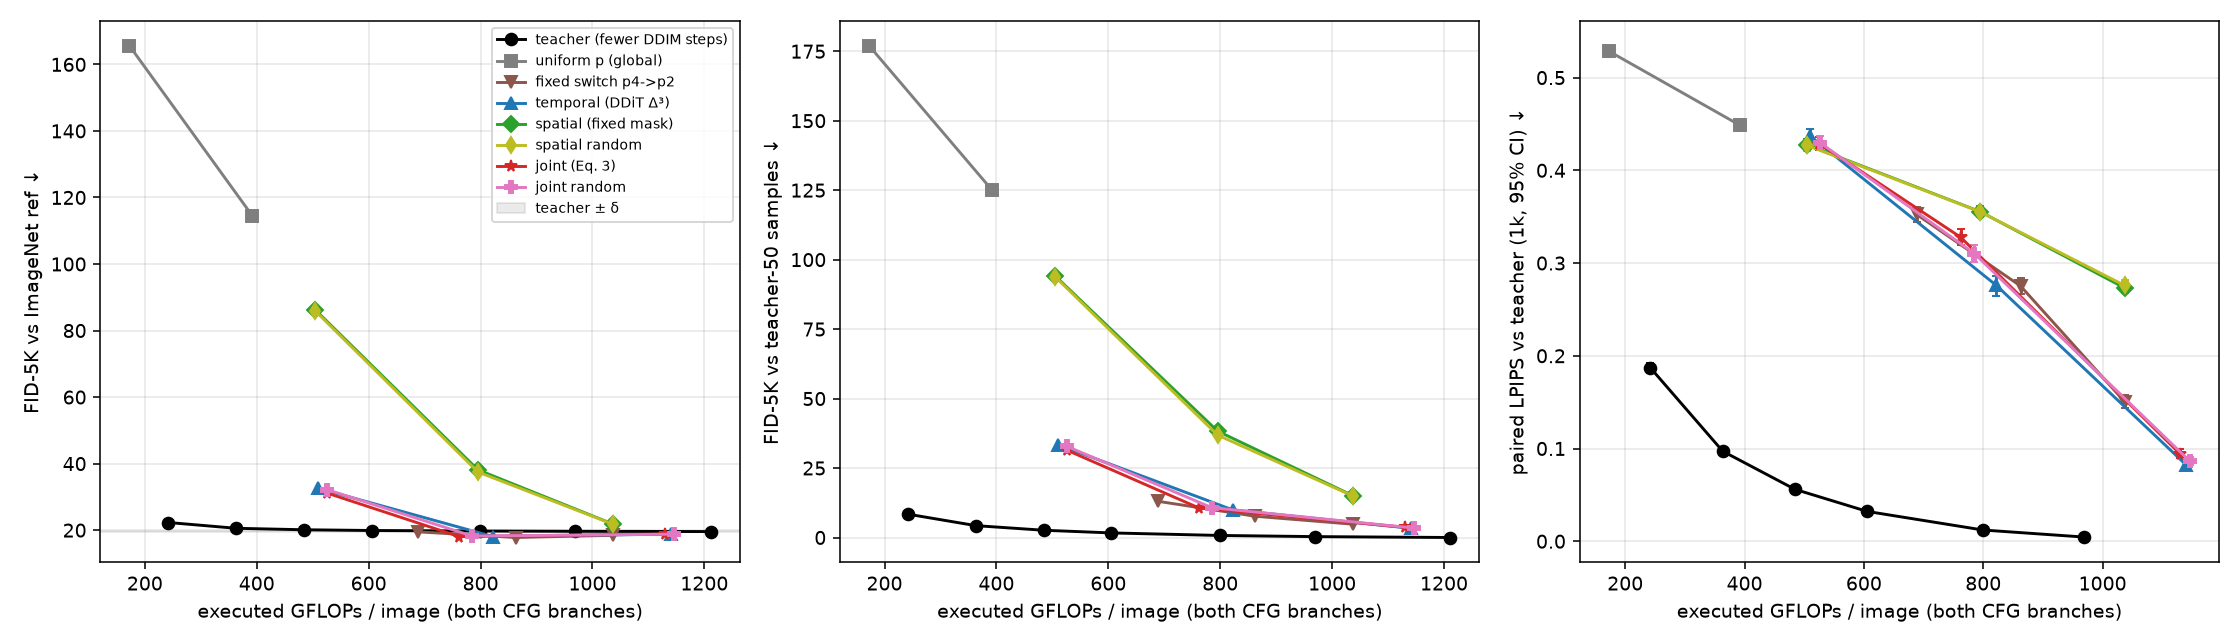
\includegraphics[width=\linewidth]{pareto.png}
\caption{Quality vs.\ executed GFLOPs per image. Left: FID-5K vs ImageNet. Middle: FID-5K vs the 50-step teacher's samples.
Right: paired LPIPS vs teacher (95\% CI). Black: the teacher with fewer DDIM steps.}
\label{fig:pareto}
\end{figure}

\begin{table}[t]
\centering
\small
\caption{Paired LPIPS differences on the same 1,000 seeds (95\% bootstrap CI). Negative means the first condition is closer to the
teacher.}
\label{tab:contrasts}
\begin{tabular}{lrrr}
\toprule
Contrast & $\sim$200--228 tok & $\sim$150--166 tok & $\sim$100 tok \\
\midrule
Joint $-$ temporal & $+0.012$ [$+0.009$, $+0.015$] & $+0.052$ [$+0.045$, $+0.060$]$^*$ & $-0.008$ [$-0.010$, $-0.007$] \\
Spatial $-$ spatial random & $-0.003$ [$-0.008$, $+0.002$] & $+0.000$ [$-0.004$, $+0.005$] & $+0.001$ [$-0.002$, $+0.004$] \\
Joint $-$ joint random & $+0.008$ [$+0.005$, $+0.011$] & $+0.018$ [$+0.014$, $+0.022$] & $-0.001$ [$-0.002$, $-0.001$] \\
\bottomrule
\end{tabular}\\[2pt]
{\footnotesize $^*$Joint used fewer tokens here (151 vs 166); compare via Figure~\ref{fig:pareto}.}
\end{table}

\subsection{Selection signals (RQ3)}
\label{sec:gap-results}
Table~\ref{tab:gap} reports the allocation gap on 256 images. Every signal ranks blocks better than random, but weakly
($\rho_S\approx0.24$--$0.31$). The training-free $\Delta^3$ score is no better than simple clean-latent variation.

The damage maps also explain the null placement result. Coarsening a single block to $p{=}8$ costs 0.151 LPIPS on average, while the
spread across the blocks of an image is only 0.065. No block is close to free to coarsen, so there is little for placement to exploit.

\begin{table}[t]
\centering
\small
\caption{Allocation gap: per-image Spearman correlation between signal and single-block coarsening damage (256 images; 95\% CI).}
\label{tab:gap}
\begin{tabular}{lrrrr}
\toprule
Signal & $\rho_S$ ($p{=}8$) & Gap ($p{=}8$) & $\rho_S$ ($p{=}4$) & Gap ($p{=}4$) \\
\midrule
$\Delta^3$, $s^{(8)}$ & 0.311 [0.275, 0.346] & 0.344 & 0.242 [0.201, 0.280] & 0.379 \\
$\Delta^3$, $s^{(4)}$ & 0.268 [0.232, 0.303] & 0.366 & 0.232 [0.194, 0.267] & 0.384 \\
$\hat x_0$ entropy & 0.281 [0.245, 0.318] & 0.359 & 0.239 [0.197, 0.278] & 0.381 \\
Clean-latent variation & 0.313 [0.273, 0.351] & 0.344 & 0.293 [0.254, 0.332] & 0.353 \\
Random & $-0.015$ [$-0.049$, 0.020] & 0.507 & $-0.008$ [$-0.040$, 0.022] & 0.504 \\
\bottomrule
\end{tabular}
\end{table}

\todo{Follow-up B (pre-registered). B1: oracle placement by measured damage vs random placement at 100 and 70 tokens on 2,000 fresh
images (go/no-go: CI upper bound $<-0.01$). B2, only if go: learned damage predictor --- allocation gap vs $\Delta^3$, and end-to-end
joint/spatial with learned placement vs random. Source: \texttt{artifacts/mixed\_eval/followup/\{oracle,learned\}.json}.}

\subsection{Aggressive budgets}
\label{sec:aggressive}
\todo{Follow-up A (pre-registered). Joint vs temporal (plus random controls) at 130/110/90/70/50 tokens on 10,000 fresh seeds.
Decision rule: joint beats temporal at a budget iff the paired-LPIPS CI upper bound $<0$, FID vs teacher is lower, and joint uses at most
2 more tokens; narrowed H1 holds iff this is true at $\ge3$ of the budgets $\{110,90,70,50\}$. Report regardless of outcome.
Source: \texttt{results/mixed/aggr\_report.md}.}

\subsection{Measured efficiency}
\label{sec:efficiency}
Table~\ref{tab:latency} reports measured sampling time.

At batch 1, every adapted condition is slower than the teacher (0.56--0.93$\times$). Sampling is overhead-bound at this scale: one
mixed CFG forward takes about 6.3\,ms at any token count, against 3.5\,ms for the teacher's 256-token forward. The extra cost comes from
embedding at all patch sizes, padding and masking, and the decoder.

At batch 256 in FP32, token reduction does buy real speed: $5.8\times$ for uniform $p{=}8$ and 1.4--2.0$\times$ for the 100-token
schedules, but only where quality is poor. The 25-step teacher is $2.0\times$ faster at LPIPS 0.032.

These numbers mean DiT-S at 256px is not a regime where cutting tokens can pay off: there are only 256 tokens, and attention is
about 11\% of FLOPs.

\todo{Stage 0 (pre-registered): trunk-only compute headroom at 256 / 1024 / 2048\,px (DiT-S/2, PixArt-$\alpha$ 1024, PixArt-$\Sigma$ 2K):
executed FLOPs, attention share, and measured speedup at 75/50/25/6\% of tokens. Gate for building the 1024\,px study: $\ge1.5\times$
at 50\% tokens. Source: \texttt{results/mixed/stage0\_headroom.md}.}

\begin{table}[t]
\centering
\small
\caption{Measured 50-step sampling speed relative to the 50-step teacher (NVIDIA B200, including the selector).}
\label{tab:latency}
\begin{tabular}{lrrr}
\toprule
Condition & FP32, batch 1 & FP32, batch 256 & bf16, batch 256 \\
\midrule
Teacher, 25 steps & 1.99$\times$ & 2.00$\times$ & 2.00$\times$ \\
Uniform $p{=}4$ / $p{=}8$ & 0.60 / 0.60$\times$ & 2.65 / 5.76$\times$ & 1.36 / 2.67$\times$ \\
Temporal, 228 / 166 / 99 tok & 0.83 / 0.68 / 0.65$\times$ & 0.91 / 0.89 / 1.68$\times$ & 0.99 / 0.99 / 0.99$\times$ \\
Joint, 226 / 151 / 101 tok & 0.78 / 0.68 / 0.63$\times$ & 0.90 / 0.91 / 1.43$\times$ & 0.99 / 0.99 / 0.86$\times$ \\
Spatial, 200 / 155 / 98 tok & 0.57 / 0.57 / 0.56$\times$ & 1.03 / 1.33 / 2.02$\times$ & 0.57 / 0.72 / 1.07$\times$ \\
\bottomrule
\end{tabular}
\end{table}
